\section{AVSLibrary}

AVSLibrary'et er en samling af custom Psoc4 komponenter, 
der gør det lettere at overskue og udvikle selve Kar, Sensor Ø og Fieldsensor. 
Der er mange ting der bliver lettere, hvis ventilerne skal inverte signalet, 
er det et enkelt sted dette skal ændres, og så bliver det rettet i alle andre 
projekter hvor de bruges. Der er også begrænsninger med hensynt til at have 
shared kode. Enums og Struct er fælles på tværs af komponenterne, for at 
sikre at Enums har de rigtige værdier og Structs er lettere at håndtere et 
samlet sted. Fieldsensor er blevet meget strømlinet via dette, da man 
blot indsætter en SensorBus, konfigurerer I2C adresse og sætter den til 
at være Fieldsensor. Derefter skal mainloopet blot opdateret high og low 
værdierne, samt kalde Communicate funktionen. Skulle I2C delen udskiftes 
med en anden bus ville det kunne gøres uden at påvirke de enkelte Fieldsensors. 
De vil blot få den nye bus med næste gang den kompileres.
Selve komponenterne er skrevet i noget "meta" c kode, da der er nogle 
specielle Psoc macro koder der bruges til at generere den færdige c kode 
for komponenten. Hvor den mest brugte er `\$INSTANCE\_NAME` som erstattes 
af det navn brugeren vælger for komponenten, derfor bør alle metoder og variabler 
prefikses med dette. Dette sikrer at alle metoder og variabler er unikke, når 
c koden genereres af brugeren. \footnote{\citet{cypress:psoc4author}}

\subsection{DebugUart}
\subsubsection{Formål}
Denne komponents formål er at overtage 
printf funktionen, og sende data strømmen fra denne ud 
via en UART. Ideen er at programmet kan kompileres med 
og uden debug. Hvis debug er deaktiveret bliver printf 
data strømmen sendt i et sort hul, ellers bliver det 
sendt ud af en UART. Dette gør at andre komponenter 
blot skal inludere en header fil, og kan derefter bruge 
printf uden at skulle tænke videre over det. Desuden giver 
komponenten også mulighed for andre komponenter at koble 
sig på en debug menu, så man kan sende kommandoer direkte 
til de individuelle komponenter. Dette er gjort via 
funktiones pointere. Når en anden komponent bliver tilføjet 
bliver denne automatisk givet et nummer i menuen. Når et 
nummer bliver indtastet skifter DebugHandle til denne 
komponent. Brugeren kan derefter bruge ESC for at komme 
tilbage til menuen og vælge en ny DebugHandle.

\StateDiagram{0.82}{AVSLibrary}{DebugMenu}

\subsubsection{Funktioner}

\funk{int Debug\_printf(const char* string, ...)}
{Er dokumenteret her, da det er en fri funktion, men hører til denne komponent.}
{Success: Antal chars udskrevet Failure: Negative number}

\funk{void Debug\_Start(void)}
{Kobler UART'ens PutString til printf funktionen. Samt starter denne op.}
{Void}

\funk{void Debug\_PutChar(char8 txDataByte)}
{Wrapper for UART\_PutChar}
{Void}

\funk{void Debug\_PutString(const char8 string[])}
{Wrapper for UART\_PutString}
{Void}

\funk{void Debug\_Communicate()}
{Redirecter input chars fra UART til den valgte DebugHandle}
{Void}

\funk{void Debug\_DebugHandle(const char ch)}
{Bruges til at skifte DebugHandle og udskrive en liste af Komponenter der er tilkoblet debug}
{Void}

\funk{void Debug\_AddComponent(void (*debugchar) (char))}
{Tilføjer en DebugHandle funktion, bruges til at koble komponenters DebugHandle til.}
{Void}



\subsection{Doseringspumpe}
%!TEX root = ../../main.tex

\section{Vandpumpe}
Til styring af dosering fra karret, anvendes en 12V inline pumpe  med tilhørende MOSFET-styringskreds. 
Vandpumpen virker ved at der påtrykkes en DC-middelspænding i form af et PWM-signal, herved kan styrken reguleres ved at justere dutycycle på PWM-signalet.
Den implementerede styringskreds ses på figur \ref{screenshot:Styringskreds} på side \pageref{screenshot:Styringskreds}, her forklares kredsløbet yderligere.
I databladet\footnote{\citet{biltema:inlinepump}} er opgivet at pumpen benytter 12V, og trækker 3A, dette giver en beregnet afsat effekt på 36W, se beregning herunder:

\begin{figure}[!h]
    \begin{align*}
        I &= 3 A \\ 
        V &= 12 V \\
        P &= I*V \\ 
        &= 36W
    \end{align*}
\label{eq:PumpeA}
\caption{Beregning af effekt i vandpumpen}
\end{figure}

Derudover er den interne modstand beregnet til:

\begin{figure}[!h]
	\begin{align*}
   		V &= 12 V \\ 
        I &= 3 A \\
        R &= \frac{V}{I} \\ 
        &= 4 \Omega
  	\end{align*}
\label{eq:pumpeOhm}
\caption{Beregning af indre modstand}
\end{figure}

Styringskredsen skal på baggrund af disse data designes til at håndtere en strøm på 3A, og en spænding på 12V. 


\newpage
\subsection{MOSFET-styringskreds}
Til kontrolkredsen er valgt at benytte en N-channel IRLZ44Z-MOSFET transistor i common-source-konfiguration. Denne type transistor er logic-level kompatibel, og har spænding/strøm-grænseværdier der opfylder kravene ovenfor.  
Logic-level kompatible betyder at $ V_{GS(th)} < 5V $ og derved kan MOSFET'en, alene drives fra en MCU, her en PSoC.
$ V_{GS(th)} $ er den threshold-spænding hvor transistoren går ”on”.


Det ses af grafen på figur \ref{screenshot:GateToSourceVoltage} at MOSFET'en ved en $ V_{GS} = 5V $, (ved $T_J = 25)$ tillader en strøm på 100A, dette er mere end rigeligt til opgaven.

\begin{figure}[!h]
	\centering
	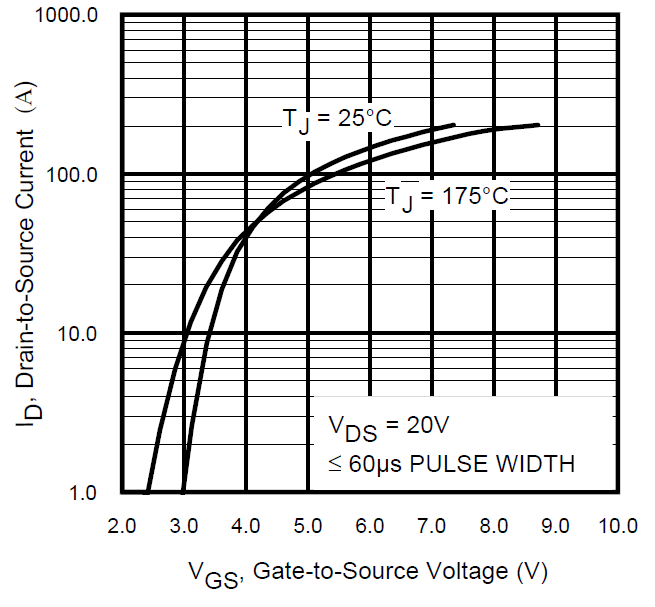
\includegraphics[scale=0.3]{../Hardware/Doseringspumpe/Screenshots/DatasheetGateToSourceVoltage}
	\caption{Datablad: Gate to Source voltage, fra databladets (Fig. 3, s.3)}
	\label{screenshot:GateToSourceVoltage}
\end{figure}

Ydermere kan det være interessant at se på hvor varm transistoren bliver under operation. Herved kan det udledes om der behøves ekstern køling eks. i form af en heat-sink.
Følgende værdier hentet fra databladet: 

\begin{figure}[!h]
	\begin{center}
		\begin{tabular}{ l l }
			 Drain to Source modstand:          & $R_{DS}=11 m\Omega$ \\ 
			 Strøm der trækkes af af relæet:    & $I = 3 A$ \\  
			 Junction-to-Ambient modstand:      & $R_{\theta JA}=62 C/W$ \\   
			 Max junction temp:                 & $Temp_{jun}=175 C$ \\
			 Ambient temp:                      & $Temp_{amb}=25 C$ \\
		\end{tabular}
	\end{center}
\caption{Værdier hentet fra datablad}
\end{figure}

Til beregningen benyttes formlen for afsat effekt: 

\begin{figure}[!h]
	\begin{align*}
		P_{afsat} &= R_{DS}*I^2 \\ 
		&= 99 mW
	\end{align*}
\caption{Afsat effekt i MOSFET}
\label{eq:afsatEffektMOSFET}
\end{figure}

Her ses det at under operation af pumpen afgiver transistoren 99 mW i varme. Ydermere noteres det, at den maksimale effekt der kan afsættes uden at der behøves heat-sink er 447.561mW. 

\begin{figure}[!h]
		\begin{align*}
			Temp_{max} &= \frac{(Temp_{jun}-Temp_{amb})}{R_{\theta JA}} \\ 
			&= 447.561 mW
		\end{align*}
\label{eq:maxMOSFETeffekt}
\caption{Max Temperatur uden heat-sink}
\end{figure}

Da der kun afsættes 99mW ved operation, er der ingen grund til at implementerer en heat-sink.

\subsubsection{Design af styringskredsløb}
På figur \ref{screenshot:Styringskreds}, ses MOSFET-styringskredsløb, PSoC'ens ”0” og ”1” er her simuleret ved en frekvensgenerator med tilpas lav frekvens.

\begin{figure}[!h]
	\centering
	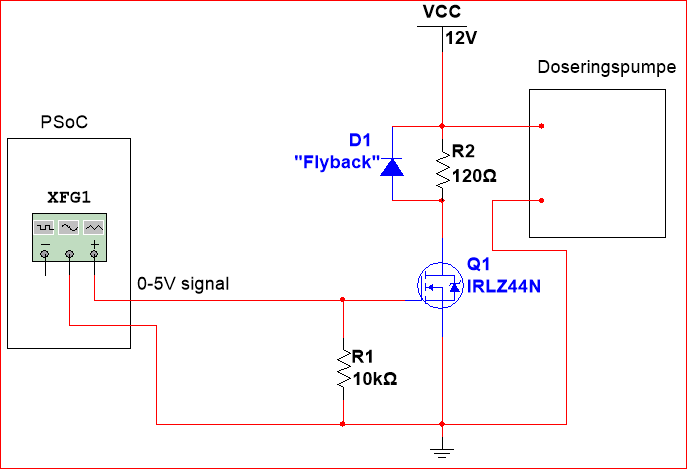
\includegraphics[height=7cm]{../Hardware/Doseringspumpe/Screenshots/DoseringspumpeStyringskredslob}
	\caption{Styringskredsløb til vandpumpe}
	\label{screenshot:Styringskreds}
\end{figure}

\paragraph{MOSFET-transistoren} \hspace{0pt} \\
Transistoren implementeres i common-source-konfiguration, for at et positivt signal på GATE til ”åbner” transistoren, og da den er en logic level model, stammer signalet direkte fra PSoC'en. 

\paragraph{Ground-modstanden} \hspace{0pt} \\
Der implementeres en modstand $R_1$ fra Gate til GND for at transistoren forbliver lukket (Gate trækkes til GND) hvis indgangssignalet til Gate afbrydes, dermed undgås det at GATE-signalet ”flyver” og transistoren potentielt kan stå og switche on/off hvis GATE afbrydes. $R_1$ implementeres med en $10k\Omega$s modstand, og virker som en standard ”pull down” resistor.

\paragraph{Flyback-diode} \hspace{0pt} \\
Derudover implementeres der, som førnævnt en ”flyback” diode, for at give strømmen en løbebane når relæet afbrydes. På denne måde indgås den høje $V_peak$ som spolen eller ville inducere, når der lukkes af for strømmen ændres monumentalt. Typen af diode, vælges ud fra følgende parametre:


\begin{description}
 \item[•] Hvilken strøm vil løbe i dioden
 \item[•] Hvilken Peak-spænding vil være over dioden
\end{description}

\subparagraph{Diode-strøm} \hspace{0pt} \\
Strømmen der vil løbe i dioden er givet fra databladet til  3A, derved skal den valgte diode kunne klare at lede max 3A, dette sker i forhold til spolens tidskonstant, $\tau$, hvor efter strømmen vil falde i løbet af $ 5 \tau$.

\subparagraph{Peak-spænding} \hspace{0pt} \\
Peak-spændingen fra spolen er realiseret i laboratoriet til 60V. \\ 

På baggrund af disse 2 værdier, vælges 1N4007, denne diode er, ifølge databladet i stand til at klare 1kVp, og 30A. Dette er tilstrækkeligt i denne situation.


\subsection{FlowSensor}
\subsubsection{Flowsensor}

\subsection{pHProbe}
\subsubsection{pHProbe}

\subsection{RS485}
\subsubsection{Formål}
Denne komponent er en UART udbygget til at virke via en RS485 bus. 
Der er tilføjet en TX Pin der skal være høj under transmission, og 
ellers lav. UARTen er bygget via interrupts og buffer, 
hvilket sikre bedre mod tab af beskedr. TX benet er implementeret ved 
at disable RX og enable TX, tænde for TX Pin og vente 20 ms. Derefter 
sende komandoen samt eventuelle argumenter. Når alt er sendt disables 
TX Pin, samt enables RX og TX disables. Da der ingen collison detection 
er, er protokollen lavet til at kun masteren snakker, og slaves kun 
svarer når master forventer dette. Modtagelsen af beskeder sker via interrupts 
og det er først relevant at kalde RS485\_GetRxMessage når beskeden er helt 
modtaget. Mark Space adresseringen er indbygget i UART komponenten, eller 
er modtage statemachinen ca det samme som kan ses under \ref{fig:RS485RX_StateDiagram}. 
Afsendelsen er lidt mere kompliceret, da afsendelsen af UART beskederne sker 
i hardwaren og ikke software. Derfor er vi nød til at aktivere interrupts 
når sender bufferen er tom, og først derefter slukke for TX benet.

\StateDiagram{0.82}{AVSLibrary}{RS485TX}

\subsubsection{Funktioner}

\funk{void RS485\_Start(void)}
{Initialiserer den underlæggende UART samt 
TX Pin'en, og klargører buffere}
{Void}
{}

\funk{void RS485\_SetAddress(uint8 addr)}
{Skifter addresse på interfacet}
{Void}
{
\funkArg{addr}{Den nye adresse der skal benyttes}
}

\funk{uint8 RS485\_GetAddress(}
{Henter adresse på interfacet}
{Adressen}
{}

\funk{uint8 RS485\_ReadRxStatus()}
{Angiver hvad status er i forhold til at der ligger en besked i bufferen}
{RS485\_MSG\_EMPTY, RS485\_MSG\_READY er de to vigtigste}
{}

\funk{void RS485\_GetRxMessage(RS485\_MSG\_STRUCT *msg)}
{Returnerer en modtaget besked, beskeden ligger stadig i bufferen og skal behandles inden den næste modtages}
{Void}
{
\funkArg{msg}{Pointer til en msg struct, som blot er pointere til forskellige steder i bufferen}
}

\funk{void RS485\_ClearRxMessage()}
{Skal køres når en besked er parset, dette gør at interfacet igen kan modtage en besked. Det gør også at værdierne i beskedn ikke længere kan forvente at være korrekte}
{Void}
{}

\funk{void  RS485\_PutTxMessage(uint8 receiver, uint8 len, uint8 cmd)}
{Sender en besked til receiver med kommandoen command, er len større end 0 skal der sendes len antal RS485\_PutTxMessageArg. Mens der sendes kan der ikke modtages beskeder. Dvs hvis der er mitchmatch mellem len og RS485\_PutTxMessageArg(uint8 arg) ender programmet i en deadlock}
{Void}
{
\funkArg{receiver}{Modtager adressen af beskeden}
\funkArg{len}{Antallet af argumenter der sendes med}
\funkArg{cmd}{Kommandoen der sendes med}
}

\funk{void RS485\_DebugHandle(const char ch)}
{Ikke implementeret endnu }
{Void}
{
\funkArg{ch}{Input char}
}

\funk{void RS485\_DebugMsg(RS485\_MSG\_STRUCT *msg)}
{Udskriver beskeden på skærmen i HEX koder, hvis debug er aktiveret bliver alle modtagne pakker udskrevet på denne måde}
{Void}
{
\funkArg{msg}{Pointer til beskeden}
}

\subsection{SensorBus}
\subsubsection{SensorBus}

\subsection{Ventil}
\subsubsection{Formål}
Formålet med denne komponent er at lave en ens 
tilgang til alle ventiler. Den indeholder en Pin, 
som kan sættes logisk høj (1) eller logisk lav(0). 
Pin signalet bliver routed til en udgang på psoc'en, 
som den styrekredsen til Ventil kan aflæse og derefter 
ændre ventil staten. I bund og grund en simpel wrapper 
for en Pin, men med debug indbygget.

\subsubsection{Funktioner}

\funk{void Ventil\_Start(void)}
{Funktionen bruges til at initialisere Pin komponenten, og derved sikre at ventilen er lukket}
{Void}
{}

\funk{void Ventil\_SetState(uint8 state)}
{Funktionen bruges til at sende signal til at sætte staten på Pin komponenten, staten bliver forwardet direkte til denne}
{Void}
{
\funkArg{state}{0: Lukket 1: Åben}
}

\funk{uint8 state Ventil\_GetState(void)}
{Funktionen bruges til at aflæse Pin'ens state}
{0: Lukket 1: Åben}
{}

\funk{void Ventil\_DebugHandle(const char ch)}
{Debug handler, se mere under DebugUart}
{Void}
{
\funkArg{ch}{Input char}
}

\funk{void Ventil\_DebugState(void)}
{Udskriver hvilken state ventilen er i}
{Void}
{}

\subsection{StubProjects}
\subsubsection{Formål}
Der blev udviklet en del stub projekter, enten til test af komponenter eller kommunikation.

\subsubsection{Debug Tester}
Projekt til at teste Debug komponenten løbende og at den havde den ønskede funktionalitet

\subsubsection{Fieldsensor Dummy}
Projekt der kunne agere som en Fieldsensor, der blot sendte statiske værdier tilbage, blev brugt til test af sensor ø'er for at sikre at ændringer ikke påvirkede kommunikationen mellem Fieldsensor og Sensor Øen.

\subsubsection{Fieldsensor Tester}
Projekt der blev brugt til at teste Fieldsensorer efter de blev bygget, for at teste om de gav korrekte værdier tilbage og om Fieldsensoren endte i deadlocks mm.

\subsubsection{FlowSensor Dummy}
Projekt til at teste og udvikle Flowsensor komponenten med udenfor Karet.

\subsubsection{pHProbe Dummy}
Projekt til at teste og udvikle pHProben komponenten med udenfor Karet.

\subsubsection{RS485 Dummy}
Projekt til at agere endpoint i RS485 kommunikations tests, den har få kommandoer indkodet og er til at teste selve protokollen og ikke kommandoerne. Derved kunne der testes fra andre platforme før selve Karret var færdig bygget. Blev også brugt til at udvikle RS485 komponenten.

\subsubsection{SensorBus Dummy}
Projekt til at agere endpoint i SensorBus kommunikations tests. Blev også brugt til at udvikle SensorBus komponenten.